\section{Moravec}\label{sec:moravec}
%Moravecs hjørnedetektor\cite{moravec}, er en af de tidligste feature detektorer og i denne metode defineres et hjørne, som et dataindsamlingsvindue i et billede $I$, der er forskelligt fra dets lokalområde. <?>
Moravecs hjørnedetektor\cite{moravec}, er en af de tidligste feature detektorer. Moravec definere et hjørne ved at placere et kvadratisk dataindsamlingsvindue over et punkt, hvorefter dette vindue forskydes med én pixel i alle principielle retninger (horisontalt, vertikalt, diagonalt). Forskellen imellem det originale og de forskudte vinduer observeres, og en stor forskel imellem vinduerne indikere et hjørne. Moravec definere altså et hjørne som værende et område, hvori der forekommer store ændringer. Forskellen imellem de forskudte vinduer defineres ved at estimere auto-korrelationen imellem det originale og de forskudte vindue. Denne auto-korrelation, eller intensitetvariation, estimeres ved SSD (Summed Square Difference):
\begin{equation}
\bold{E}_{u,v}(x,y)= \sum_{\forall \text{x,y i dataindsamlingsvinduet}} w(x,y)[I(x+u,y+v) - I(x,y)]^2
\label{moravec}     
\end{equation}
hvor $(u,v)\in \lbrace -1,0,1 \rbrace$ er sættet af forskydninger af vinduet.
%<$w$ er her en matrix<?>, med samme størrelse som $I$ <??> og indeholder 1 indenfor hvis en pixelkoordinat $(x,y)$ ligger indenfor dataindsamlingsvinduet, og 0 ellers<?>.>
Figur \ref{fig:moravec} illustrere et dataindsamlingsvindue af størrelse $3\times3$ (markeret med rød). Det blå vindue viser et diagonalt skift af dataindsamlingsvinduet med $(u,v)=(1,1)$, placeret på en pixel, der står i kontrast til dens baggrund og et vindue placeret på et hjørne. Forskydes vinduet, placeret på den enelige pixel, vil intensitetsvariation være ens for alle forskydninger. Deformationer i billedet som støj kan derved fejlagtigt detekteres som hjørner.
\begin{figure}[H]
    \centering
    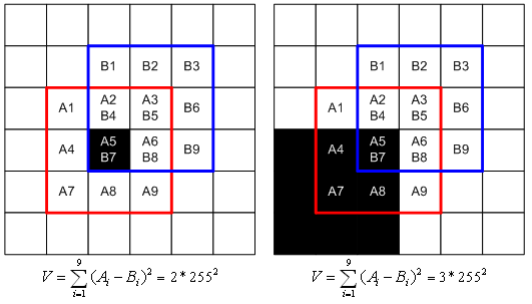
\includegraphics[width=0.55\textwidth]{fig/25.png}
     \vspace{-1em}
    \begin{center}    
       \caption{\textcolor{gray}{\footnotesize \textit{SSD udregninger for to forskellige scener. (venstre) et dataindsamlingsvindue placeret på en mørk pixel. (højre) et dataindsamlingsvindue placeret et hjørne. }}}
    \label{fig:moravec}
     \end{center}
     \vspace{-2.5em}
  \end{figure} \noindent   
$E(x,y)$ består af otte værdier, da hvert skift $(u,v)$ returnere en intensitetsvariation. Den mindste af de otte variationer, definere punktets hjørnestyrke $C(x,y)$.
$$
C(x,y)=min(\bold{E}_{u,v}(x,y)) \forall S_{(u,v)} \in \lbrace-1,0,1\rbrace \backslash \lbrace0,0\rbrace
$$
En horisontal kant vil resultere i en lav intensitetsvariation med et dataindsamlingsvindue forskudt horisontalt derfor, for at identificere hjørner, tages minimum af $\bold{E}$ for at sikre en stor auto-korrelation i alle retninger.
%<vil have et højt respons i de områder, hvor pixelintensiteter i originalvinduet ($w(x,y) = 1$) <?>, adskiller sig fra intensiteter, i de forskudte vinduer - jo større pixelintensitens forskellen er, jo højere $C$ værdi.
Det kan udledes her, at en kant, med retning i en de principielle retninger, ikke vil blive karakteriseret som et hjørne da disse vil have  en lav auto-korrelation. Der opstilles en grænseværdi $t$ for $C$, der bestemmer om punktet er et hjørne(sandt/falsk) og derved om det kan udvælges som et interessepunkt.
\begin{equation}
\begin{split}
\text{hjørne} = 
\begin{cases}
\text{sandt}& \text{hvis } C(x,y)\geq t, \\
\text{falsk }& \text{hvis } C(x,y) < t.
\end{cases}
\end{split}
\label{cornerind}
\end{equation}
Moravec lider af følgende problemer pga. dens simplicitet:
\begin{itemize}
\item{Der undersøges kun et diskret sæt af pixelskift (i hver principiel retning) og resultatet er derfor anisotropisk, (afhængig af retning). Undersøges en kant, der ikke er horisontal, vertikal eller diagonal, vil den mindste intensitetsvariation være stor, og derved kan punktet fejlagtigt detekteres som et hjørne.}
\item{Det skiftende vindue er rektangulært, og metoden er derfor meget følsom overfor støj i billedet.}
\item{Detektoren finder punkter lokaliseret på kanter. Små deformationer i kanterne som støj, vil resultere i at den mindste intensitetsvariation vil være relativt stor, og derfor detektere punktet som værende et interessepunkt.}
\end{itemize}
\subsection{Algoritme}
\begin{enumerate}
\item{For hvert pixel i billedet, udregn auto-korrelationen imellem skift af $(u,v) \in \lbrace-1,0,1\rbrace$. udregnet ved ligning \ref{moravec}}
\item{\textit{Find "Hjørnestyrken"} ved at tage $C(x,y)=min(\bold{E}_{u,v}(x,y))$}
\item{Fjern punkter der ikke overholder en sat grænseværdi for $C(x,y)$.}
\end{enumerate}
\subsection{Konklusion}
Moravec er som nævnt en simpel algoritme, med mange udfordringer, der gør at den ikke bruges som en repeterbar detektor. Detektoren er i dag ikke i sig selv relevant, som den var da den blev udgivet, men bygges videre på i andre detektorer, f.eks. \cite{Harris} beskrevet i sektion, \ref{sec:harris} som direkte tilgår de nævne problemstillinger med Moravec.